% CSE558 Midterm Project Report, laid out like the course template (CSE558_Project_Report_Template.pdf).
% Overleaf: upload this file as main.tex and the 8 PDFs from figures/ into a folder named figures; compile with pdfLaTeX.
% Every number below is copied from the printed output of notebooks/midterm.ipynb.
\documentclass[10pt,a4paper,twocolumn]{article}

\newif\ifshowhints
\showhintsfalse   % hints hidden for submission; \showhintstrue shows the template's grey instructions again
\newcommand{\projecttitle}{Is a wine's score about the wine or the critic? Hypothesis tests on 120k wine reviews}

\usepackage[T1]{fontenc}
\usepackage[utf8]{inputenc}
\usepackage[default]{lato}
\usepackage[left=18mm,right=18mm,top=18mm,bottom=22mm,columnsep=7mm]{geometry}
\usepackage{amsmath}
\usepackage{graphicx}
\usepackage{xcolor}
\usepackage{array}
\usepackage{booktabs}
\usepackage{tabularx}
\usepackage{enumitem}
\usepackage[font=small,labelfont=bf]{caption}
\usepackage{titlesec}
\usepackage{microtype}
\usepackage[hidelinks]{hyperref}

\graphicspath{{figures/}{../figures/}}
\setlength{\parindent}{0pt}
\setlength{\parskip}{4pt}
\setlength{\tabcolsep}{4pt}
\setlist{nosep,leftmargin=*}
\raggedbottom   % leave space at the bottom of a column instead of stretching gaps between paragraphs

\newcolumntype{L}{>{\raggedright\arraybackslash}X}
\newcolumntype{P}[1]{>{\raggedright\arraybackslash}p{#1}}
\newcolumntype{H}{>{\bfseries\boldmath\raggedright\arraybackslash}p{30mm}}

\titleformat{\section}{\large\bfseries}{\thesection.}{0.4em}{}
\titlespacing*{\section}{0pt}{10pt}{3pt}
\titleformat{\subsection}{\normalsize\bfseries}{}{0pt}{}
\titlespacing*{\subsection}{0pt}{8pt}{2pt}
\titleformat{\subsubsection}{\normalsize\bfseries}{}{0pt}{}
\titlespacing*{\subsubsection}{0pt}{5pt}{1pt}

\newcommand{\hint}[1]{\ifshowhints\par{\color{gray}\itshape\small #1\par}\fi}
\newcommand{\col}[1]{\texttt{\detokenize{#1}}}
% a figure that stays where it is written: the plot, then its one-line takeaway as the caption
\newcommand{\plotfig}[2]{\par\smallskip\noindent\begin{minipage}{\columnwidth}\centering
  \includegraphics[width=\columnwidth]{#1}\captionof{figure}{#2}\end{minipage}\par\smallskip}

\begin{document}

\twocolumn[{%
{\small\bfseries CSE558 Data Science $\bullet$ Midterm Project Report $\bullet$ Monsoon 2026}\par
\vspace{8pt}
{\LARGE\bfseries \projecttitle\par}
\vspace{8pt}
\noindent\rule{\textwidth}{0.4pt}\par
\hint{Everything in light blue is a worked example: replace it with your own. Grey italic lines are instructions: delete
them, or hide them all with \textbackslash showhintsfalse. Sections 1--5 follow items 1--5 of the report guidelines;
Section 6 is the limitations of your analysis. At most 8 pages.}
\vspace{2pt}
\noindent\begin{tabular}{@{}P{30mm}l@{}}
\textbf{Group name} & Data Brokers\\
\textbf{Dataset} & \href{https://www.kaggle.com/datasets/zynicide/wine-reviews}{kaggle.com/datasets/zynicide/wine-reviews}\\
\textbf{Code} & \href{https://github.com/hhiten10/DATA_BROKERS_DSC}{github.com/hhiten10/DATA\_BROKERS\_DSC} (notebook and README)\\
\end{tabular}\par
\hint{Code: a link to the code written by you and a readme file, which anyone with the link can open. Also upload your
notebook or script on the classroom.}
\noindent\begin{tabular}{@{}P{5mm}P{28mm}P{17mm}P{45mm}P{67mm}@{}}
\toprule
\textbf{\#} & \textbf{Name} & \textbf{Roll no.} & \textbf{Institute email} & \textbf{Contribution}\\
\midrule
1 & Himanshu & MT25068 & himanshu25068@iiitd.ac.in & With Yash: dataset, preparation, Tests 1--2 (1--3, 5).
With Ishan: Tests 4--5, limitations, code and README (5, 6)\\
2 & Yash Verma & MT25092 & yash25092@iiitd.ac.in & With Himanshu: dataset, preparation, Tests 1--2 (1--3, 5).
With Ishan: EDA, problem statements, Test 3 (4, 5)\\
3 & Ishan Agrawal & MT25025 & ishan25025@iiitd.ac.in & With Yash: EDA, problem statements, Test 3 (4, 5).
With Himanshu: Tests 4--5, limitations, code and README (5, 6)\\
\bottomrule
\end{tabular}\par
\vspace{14pt}
}]

% ---------------------------------------------------------------------------------------------------------------------
\section{Dataset}
\hint{Where you have collected the dataset, how many rows and columns there are, and whether \#instances $\times$
\#attributes is at least 3M after encoding (show the arithmetic). Name some features with their interpretation to the
real world.}

\textbf{Source:} Kaggle, ``Wine Reviews'' by zynicide, downloaded on 22 October 2026. The reviews come from
WineEnthusiast magazine and were collected in 2017. We use only \col{winemag-data-130k-v2.csv}. Each row is one review
of one wine.

\textbf{Problems in the raw data:} repeated rows, missing prices and critic names, the vintage year hidden inside the
wine's name, extra spaces in the text, the same grape under two names (Syrah and Shiraz), and a few very expensive
bottles (up to \$3,300).

{\small
\begin{tabularx}{\columnwidth}{@{}Lrr@{}}
\toprule
 & \textbf{Raw file} & \textbf{After encoding}\\
\midrule
Instances (rows) & 129,971 & 119,895\\
Attributes (columns) & 13 & 26\\
Instances $\times$ attributes & 1,689,623 & 3,117,270\\
\bottomrule
\end{tabularx}\par}

\textbf{Size check:} $119{,}895 \times 26 = 3{,}117{,}270 \geq 3{,}000{,}000$, so the requirement is met. The 26
columns are 5 number columns (\col{points}, \col{price}, \col{price_imputed}, \col{vintage}, \col{desc_words}) plus
one-hot columns for \col{country} (10) and \col{variety} (11). If we had deleted the rows with a missing price, we would
have only $111{,}511 \times 26 = 2{,}899{,}286$, which is below 3M.

\subsection*{Key features}
\hint{Some key features, with their type (nominal, discrete or continuous) and real-world meaning. Include the response
variable, if there is one.}
{\small
\begin{tabularx}{\columnwidth}{@{}P{21mm}P{15mm}L@{}}
\toprule
\textbf{Feature} & \textbf{Type} & \textbf{Real-world meaning}\\
\midrule
\col{points} & discrete & score from 80 to 100; what we study\\
\col{price} & continuous & price of the bottle in US dollars\\
\col{country} & nominal & country of the wine; 43 values\\
\col{province} & nominal & state or province, e.g.\ Washington; 425 values\\
\col{variety} & nominal & grape type; 707 values\\
\col{taster_name} & nominal & the critic who scored the wine; 19 critics\\
\col{title} & text & name of the wine; contains the vintage year\\
\col{description} & text & the critic's review; we count its words (\col{desc_words})\\
\bottomrule
\end{tabularx}\par}

% ---------------------------------------------------------------------------------------------------------------------
\begin{figure*}[t]
\centering
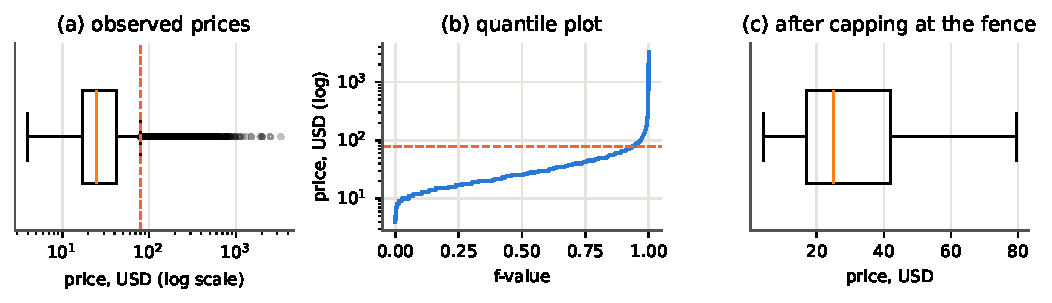
\includegraphics[width=\textwidth]{fig_price_outliers.pdf}
\caption{Prices have a long tail to the right: 6,867 bottles are above the \$79.5 fence (dashed line) and the most
expensive costs \$3,300 (a, b). After capping at the fence, the long tail is gone (c).}
\label{fig:outliers}
\end{figure*}

\section{Data preparation}
\hint{How did you prepare your data (encoding, outliers, missing values, duplicates), and why do you follow such steps?
One row per step; the ``why'' matters most.}

% the table is split in two so it can continue in the next column instead of running off the page
{\footnotesize
\begin{tabularx}{\columnwidth}{@{}P{22mm}P{24mm}L@{}}
\toprule
\textbf{Issue found} & \textbf{What we did} & \textbf{Why}\\
\midrule
9,983 rows are exact copies & removed them & the same review counted twice makes the sample look bigger than it is\\
33 reviews appear on two different wines & kept only the first & the same text should not count twice in Test 2\\
59 rows have no country, 1 has no variety & removed them & too few to matter, and we cannot guess them\\
8,384 prices are missing, more in some countries (20.0\% in France, 0.4\% in the US) & filled with the median price of
the same country; marked in \col{price_imputed}; the tests skip these rows & median, because a few very expensive
bottles pull the mean up; we keep the rows because their scores are real\\
1 in 5 reviews has no critic name & filled with \texttt{Unknown} & the review and score are still real; Tests 4--5 use
only two named critics\\
\bottomrule
\end{tabularx}\par}

{\footnotesize
\begin{tabularx}{\columnwidth}{@{}P{22mm}P{24mm}L@{}}
\toprule
\textbf{Issue found} & \textbf{What we did} & \textbf{Why}\\
\midrule
4 columns not useful: \col{region_2} (61\% missing), the Twitter handle (repeats the critic), \col{winery},
\col{designation} (too many values) & removed them & too empty, repeated, or too many values to compare groups\\
extra spaces in titles; a hidden space character in critic names & cleaned them & otherwise a search for a critic's
name misses some rows\\
the vintage year is inside the wine's name & took it out with a regex; left empty if there is no year, it says NV, or
there are two years & a wrong year is worse than an empty one\\
one grape, two names (e.g.\ Shiraz and Syrah) & merged 3 such pairs; 2,077 rows renamed & otherwise one grape is split
into two groups\\
6,867 prices above the IQR fence $Q_3 + 1.5\,\mathrm{IQR} = \$79.5$ (Figure~\ref{fig:outliers}) & capped them at
\$79.5; the original price is kept in \col{price_raw} & real luxury wines, not mistakes, so we keep them; capping stops
them pulling averages up\\
\col{country} and \col{variety} are categories & one-hot encoded the top 9 countries and top 10 varieties; the rest
became Other & numbering them 1, 2, 3 would invent an order; very small groups are unreliable\\
no column for review length & added \col{desc_words}, the number of words & needed for Test 2\\
\bottomrule
\end{tabularx}\par}

% ---------------------------------------------------------------------------------------------------------------------
\section{What changed after preparation}
\hint{What are the changes you got after data preparation? Give before-and-after observations.}

{\small
\begin{tabularx}{\columnwidth}{@{}LP{17mm}P{27mm}@{}}
\toprule
\textbf{Measure} & \textbf{Before} & \textbf{After}\\
\midrule
Rows & 129,971 & 119,895\\
Columns & 13 & 26 after encoding\\
Exact copies & 9,983 & 0\\
Reviews used twice & 33 & 0\\
Missing prices & 8,996 & 0 (8,384 filled and marked)\\
Missing critic names & 26,244 & 0 (\texttt{Unknown})\\
Grape varieties & 707 & 698\\
Prices above \$79.5 & 7,241 & 0 (capped)\\
Price kurtosis & 829.5 & 0.1\\
Vintage year & inside the name & a number for 115,529 rows\\
\bottomrule
\end{tabularx}\par}

\emph{Before} is the raw file, so its counts include the copied rows. We only removed rows that were copies or had no
country or variety; everything else was fixed and kept. Capping removed the extreme prices: kurtosis fell from 829.5 to
0.1. The new \col{vintage} and \col{desc_words} columns made Tests 2, 4 and 5 possible.

% ---------------------------------------------------------------------------------------------------------------------
\section{Basic questions and problem statement}
\hint{What are your basic questions about your data, and how is your problem statement novel from them? Show a few EDA
plots, each with a one-line takeaway.}

\plotfig{fig_points.pdf}{Scores go from 80 to 100 (mean 88.4, SD 3.1). There are none below 80 because the magazine
does not publish them. 38\% of wines score 90 or more.}

\plotfig{fig_price_points.pdf}{Pricier wines score higher: the median score rises from 86 to 93 across the price bands
(correlation of log price with score: 0.62). So we must compare wines at the same price.}

\plotfig{fig_tasters.pdf}{For \$20--40 wines, the critics' average scores differ by up to 4.9 points, so the critic may
matter as much as the wine. Orange: the two critics compared in Tests 4--5.}

\plotfig{fig_words.pdf}{Longer reviews come with higher scores (correlation 0.54): about 82 points for the shortest
reviews and 92 for the longest.}

\subsection*{Basic questions}
\begin{enumerate}
\item Do pricier wines score higher? Yes: the correlation of log price with score is 0.62.
\item Which countries score best? Austria (90.22 on average) and Germany (89.88), among countries with 500+ priced
reviews.
\item Which grapes are reviewed most? Pinot Noir (12,274), Chardonnay (10,864) and Cabernet Sauvignon (8,835).
\end{enumerate}

\subsection*{Our problem statements}
\hint{One or two sentences each, specific to your features, and phrased so each could come out either way. Mark one as
primary.}
\noindent\fbox{\parbox{\dimexpr\columnwidth-2\fboxsep-2\fboxrule\relax}{%
\textbf{P1 (main).} For the same kind of wine, does the critic change the score? We check how often two critics give
90+ (Test 4) and how spread out their scores are (Test 5).\par\smallskip
\textbf{P2.} At the same price, do Old-World wines score differently from New-World wines? (Test 1)\par\smallskip
\textbf{P3.} Do longer reviews go with higher scores? (Test 2)\par\smallskip
\textbf{P4.} At what price does a 90+ score become likely? (Test 3)}}

\textbf{How they are new:} the basic questions look at one column at a time. Our questions compare like with like
(same price, or same state and years) and need columns we made ourselves (price band, Old/New World, vintage, word
count).

% ---------------------------------------------------------------------------------------------------------------------
\section{Statistical inferences}
\hint{Conduct 3--5 hypothesis tests on your problem statement(s), each with parts a)--c) below. Know your tests and the
reason for using them, and compare them with other tests.}

\textbf{Rows tested:} the 111,511 reviews with a real price; the 8,384 filled-in prices are left out. We use
$\alpha = 0.05$ and 95\% confidence intervals (CIs). With this many rows, even a tiny difference is significant. So
before each test we decide the smallest difference that would matter in real life, and after the test we compare the CI
with it: \emph{matters} if the whole CI is beyond it, \emph{does not matter} if the whole CI is inside it, and
\emph{unclear} if the CI crosses it.

% ----- Test 1 -----
\subsection*{Test 1 (P2): Old-World vs New-World wines at \$20--40}

\subsubsection*{a) Hypotheses, written before running the test}
\hint{Before running the test, write the null and alternative hypotheses ($H_0$ carries the equality), the
significance level, one- or two-sided, the test you will use, and the smallest difference that would matter in the
real world.}
{\small
\begin{tabularx}{\columnwidth}{@{}HL@{}}
\toprule
$H_0$ & $\mu_{\text{Old}} - \mu_{\text{New}} = 0$\\
$H_1$ & $\mu_{\text{Old}} - \mu_{\text{New}} \neq 0$\\
Significance level & $\alpha = 0.05$\\
Side & two-sided\\
Test & two-sample t-test (an F-test first checks if the variances are equal)\\
Smallest difference that matters & 1 point\\
\bottomrule
\end{tabularx}\par}

$\mu_{\text{Old}}, \mu_{\text{New}}$: average score of \$20--40 wines from the Old World (Europe and nearby countries
such as Israel and Georgia) and the New World (the Americas, Australia, New Zealand, South Africa). Two-sided, because
we did not guess a direction. 1 point, because scores are whole numbers, so a smaller gap would not change a printed
score. Groups: 18,047 Old-World and 27,929 New-World wines.

\subsubsection*{b) Other tests we considered}
\hint{Which other tests did you consider, and why did you not use them? Say first why your test fits your data.}
Two separate groups, a score that is a number, and an unknown $\sigma$: so a two-sample t-test. The F-test says the
variances are not equal ($F = 0.765$, $p = 7.94 \times 10^{-86}$), so we use Welch's t-test, which does not need equal
variances.

{\footnotesize
\begin{tabularx}{\columnwidth}{@{}P{23mm}L@{}}
\toprule
\textbf{Also considered} & \textbf{Why we did not use it}\\
\midrule
Pooled t-test & assumes equal variances, which is not true here. We ran it anyway: $t = 23.95$, same decision\\
Two-sample z-test & needs the true $\sigma$, which we do not know\\
Paired t-test & no wine is in both groups, so there is nothing to pair\\
$\chi^2$ test & would only use 90+ yes/no and lose the exact score\\
\bottomrule
\end{tabularx}\par}

\subsubsection*{c) Result}
\hint{Report the test statistic, degrees of freedom, p-value and decision, and the estimate with a 95\% confidence
interval. Is the difference large enough to matter?}
{\small
\begin{tabularx}{\columnwidth}{@{}HL@{}}
\toprule
Estimate & $+0.595$ point (88.828 Old World, 88.232 New World)\\
95\% confidence interval & 0.548 to 0.643\\
Test statistic (d.f.) & $t = 24.64$ (42,033)\\
p-value & $3.84 \times 10^{-133}$\\
Decision & reject $H_0$\\
\bottomrule
\end{tabularx}\par}

Old-World wines score a little higher, and the difference is real. But the whole CI is below 1 point, so it
\textbf{does not matter} in practice.

% ----- Test 2 -----
\subsection*{Test 2 (P3): longer reviews vs higher scores}

\subsubsection*{a) Hypotheses, written before running the test}
{\small
\begin{tabularx}{\columnwidth}{@{}HL@{}}
\toprule
$H_0$ & $\rho \leq 0$\\
$H_1$ & $\rho > 0$\\
Significance level & $\alpha = 0.05$\\
Side & one-sided (right)\\
Test & t-test on the correlation $r$, df $= n - 2$\\
Smallest effect that matters & $\rho = 0.3$\\
\bottomrule
\end{tabularx}\par}

$\rho$: correlation between the number of words in a review and its score. One-sided, because P3 asks about
\emph{higher} scores. 0.3, because a smaller correlation explains less than 9\% of the score ($0.3^2 = 0.09$).

\subsubsection*{b) Other tests we considered}
Both are numbers measured on the same review, so we test their correlation with a t-test.

{\footnotesize
\begin{tabularx}{\columnwidth}{@{}P{23mm}L@{}}
\toprule
\textbf{Also considered} & \textbf{Why we did not use it}\\
\midrule
Welch t-test, long vs short reviews & a rougher question (reviews split at the median length). We ran it: long reviews
score 2.694 points higher (CI 2.661 to 2.727), same decision\\
$\chi^2$ test & would need us to cut review length into groups\\
Paired t-test & nothing to pair\\
\bottomrule
\end{tabularx}\par}

\subsubsection*{c) Result}
{\small
\begin{tabularx}{\columnwidth}{@{}HL@{}}
\toprule
Estimate & $r = 0.538$\\
95\% confidence interval & 0.534 to 0.542\\
Test statistic (d.f.) & $t = 213.07$ (111,509)\\
p-value & $\approx 0$\\
Decision & reject $H_0$\\
\bottomrule
\end{tabularx}\par}

The whole CI is above 0.3, so it \textbf{matters}: longer reviews go with higher scores. This does not mean long
reviews cause high scores; critics probably write more about wines they like.

% ----- Test 3 -----
\subsection*{Test 3 (P4): price band vs the chance of a 90+ score}

\subsubsection*{a) Hypotheses, written before running the test}
{\small
\begin{tabularx}{\columnwidth}{@{}HL@{}}
\toprule
$H_0$ & the chance of 90+ is the same in every price band\\
$H_1$ & the chance of 90+ differs between bands\\
Significance level & $\alpha = 0.05$\\
Side & one-sided (a $\chi^2$ test uses the upper tail)\\
Test & $\chi^2$ test for independence, df $= (5-1)(2-1) = 4$\\
Smallest difference that matters & 5 percentage points between neighbouring bands\\
\bottomrule
\end{tabularx}\par}

Price bands: up to \$15, \$15--25, \$25--40, \$40--79.5 and over \$79.5. 5 percentage points (pp) means one more 90+
wine in every 20.

\subsubsection*{b) Other tests we considered}
Price band and 90+ (yes/no) are both categories, so we use the $\chi^2$ test for independence. Every expected count is
at least 2,592, well above 5. A $\chi^2$ test does not give one estimate with a CI, so part c) shows the 90+ share of
each band with its CI.

{\footnotesize
\begin{tabularx}{\columnwidth}{@{}P{23mm}L@{}}
\toprule
\textbf{Also considered} & \textbf{Why we did not use it}\\
\midrule
z-test for two proportions & compares only two bands at a time. We ran it on the cheapest vs the most expensive band:
$+80.7$ pp (CI 79.8 to 81.6)\\
$\chi^2$ goodness of fit & needs an expected distribution to compare with, and we do not have one\\
\bottomrule
\end{tabularx}\par}

\subsubsection*{c) Result}
$\chi^2 = 30{,}191.9$, df $= 4$, $p \approx 0$: reject $H_0$.

{\footnotesize
\begin{tabularx}{\columnwidth}{@{}Lrll@{}}
\toprule
\textbf{Price band} & \textbf{$n$} & \textbf{90+ share, \% (CI)} & \textbf{Step up, pp (CI)}\\
\midrule
up to \$15 & 23,256 & 5.1 (4.8 to 5.4) & --\\
\$15--25 & 33,129 & 23.4 (23.0 to 23.9) & $+18.3$ (17.8 to 18.8)\\
\$25--40 & 25,984 & 45.7 (45.1 to 46.3) & $+22.2$ (21.5 to 23.0)\\
\$40--79.5 & 22,275 & 69.1 (68.5 to 69.7) & $+23.4$ (22.6 to 24.3)\\
over \$79.5 & 6,867 & 85.8 (85.0 to 86.6) & $+16.7$ (15.7 to 17.7)\\
\bottomrule
\end{tabularx}\par}

\plotfig{fig_band90.pdf}{The chance of a 90+ score rises from 5\% to 86\% and passes one half (dashed line) in the
\$40--79.5 band.}

Each step up in price adds more than 5 pp, and every CI is above 5 pp, so all 4 steps \textbf{matter}. A 90+ score
becomes more likely than not in the \$40--79.5 band.

% ----- Test 4 -----
\subsection*{Test 4 (P1): two critics, same kind of wine: how often 90+?}

Paul Gregutt and Sean P. Sullivan both review wines from Washington State. To compare like with like, we use only
Washington wines at \$20--40 from the years both critics reviewed at least 25 times (2009--2012,
Figure~\ref{fig:vintages}). Gregutt scored 1,047 of these wines and Sullivan 806.

\plotfig{fig_wa_vintages.pdf}{The two critics reviewed Washington wines in different years. Only 2009--2012 (shaded)
has 25+ wines from both, so Tests 4 and 5 use only those years.\label{fig:vintages}}

\subsubsection*{a) Hypotheses, written before running the test}
{\small
\begin{tabularx}{\columnwidth}{@{}HL@{}}
\toprule
$H_0$ & $p_G - p_S = 0$\\
$H_1$ & $p_G - p_S \neq 0$\\
Significance level & $\alpha = 0.05$\\
Side & two-sided\\
Test & z-test for two proportions\\
Smallest difference that matters & 5 percentage points\\
\bottomrule
\end{tabularx}\par}

$p_G, p_S$: share of wines scored 90+ by Gregutt and by Sullivan. Two-sided, because we did not guess which critic is
more generous. 5 pp means one more 90+ wine in every 20.

\subsubsection*{b) Other tests we considered}
Two separate groups with a yes/no result (90+ or not), so we use the z-test for two proportions. Each group has well
over 10 wines on each side of 90, so the normal approximation is fine.

{\footnotesize
\begin{tabularx}{\columnwidth}{@{}P{23mm}L@{}}
\toprule
\textbf{Also considered} & \textbf{Why we did not use it}\\
\midrule
$\chi^2$ test on the $2 \times 2$ table & gives the same answer ($\chi^2 = 24.16 = z^2$) but no CI for the
difference\\
Welch t-test & compares average scores, which is a different question\\
Paired t-test & needs the same wines scored by both critics; only 1 of 1,851 wines was\\
\bottomrule
\end{tabularx}\par}

\subsubsection*{c) Result}
{\small
\begin{tabularx}{\columnwidth}{@{}HL@{}}
\toprule
Estimate & $+11.4$ pp (Gregutt 49.3\%, Sullivan 37.8\%)\\
95\% confidence interval & 6.9 to 16.0 pp\\
Test statistic (d.f.) & $z = 4.92$ (no d.f. for z)\\
p-value & $8.85 \times 10^{-7}$\\
Decision & reject $H_0$\\
\bottomrule
\end{tabularx}\par}

For the same kind of wine, Gregutt gives 90+ more often. The whole CI is above 5 pp, so the critic \textbf{matters}.
The years cannot explain it, because both critics are compared on the same years.

% ----- Test 5 -----
\subsection*{Test 5 (P1): two critics, same kind of wine: how spread out are the scores?}
Same wines as Test 4.

\subsubsection*{a) Hypotheses, written before running the test}
{\small
\begin{tabularx}{\columnwidth}{@{}HL@{}}
\toprule
$H_0$ & $\sigma_G^2 / \sigma_S^2 = 1$\\
$H_1$ & $\sigma_G^2 / \sigma_S^2 \neq 1$\\
Significance level & $\alpha = 0.05$\\
Side & two-sided\\
Test & F-test for two variances\\
Smallest difference that matters & SD ratio of 1.2\\
\bottomrule
\end{tabularx}\par}

$\sigma_G^2, \sigma_S^2$: variance of each critic's scores. An SD ratio of 1.2 means one critic's scores are 20\% more
spread out (about half a point), enough to move some wines across 90.

\subsubsection*{b) Other tests we considered}
We compare spread, not averages, for two separate groups, so we use the F-test for two variances. It needs roughly
normal scores; the Q-Q plots (Figure~\ref{fig:qq}) show they are close to normal.

\plotfig{fig_qq.pdf}{Both critics' scores are close to the normal line, but Sullivan's are less spread out (SD 2.15)
than Gregutt's (SD 2.54).\label{fig:qq}}

{\footnotesize
\begin{tabularx}{\columnwidth}{@{}P{23mm}L@{}}
\toprule
\textbf{Also considered} & \textbf{Why we did not use it}\\
\midrule
$\chi^2$ test for one variance & treats Gregutt's variance as exactly known, which it is not, so its p-value is too
small. We ran it: $\chi^2 = 575.60$, $p = 2.07 \times 10^{-10}$\\
z- and t-tests & compare averages, not spread\\
\bottomrule
\end{tabularx}\par}

\subsubsection*{c) Result}
{\small
\begin{tabularx}{\columnwidth}{@{}HL@{}}
\toprule
Estimate & variance ratio 1.399 (SD ratio 1.183)\\
95\% confidence interval & variance ratio 1.227 to 1.592; SD ratio 1.108 to 1.262\\
Test statistic (d.f.) & $F = 1.40$ (1,046, 805)\\
p-value & $5.54 \times 10^{-7}$\\
Decision & reject $H_0$\\
\bottomrule
\end{tabularx}\par}

Gregutt's scores are more spread out, and this is significant. But the CI for the SD ratio (1.108 to 1.262) crosses
1.2, so it is \textbf{unclear} whether the difference matters.

% ----- Summary -----
\subsection*{Summary of the five tests}
{\footnotesize
\begin{tabularx}{\columnwidth}{@{}lLP{20mm}P{13mm}P{13mm}@{}}
\toprule
 & \textbf{Question} & \textbf{Estimate (95\% CI)} & \textbf{Matters if} & \textbf{Verdict}\\
\midrule
T1 & Old vs New World, \$20--40 & $+0.595$ point (0.548 to 0.643) & 1 point & does not matter\\
T2 & review length vs score & $r = 0.538$ (0.534 to 0.542) & $r = 0.3$ & matters\\
T3 & price band vs 90+ & steps of $+16.7$ to $+23.4$ pp & 5 pp per step & all 4 steps matter\\
T4 & Gregutt vs Sullivan, 90+ share & $+11.4$ pp (6.9 to 16.0) & 5 pp & matters\\
T5 & Gregutt vs Sullivan, spread & SD ratio 1.183 (1.108 to 1.262) & SD ratio 1.2 & unclear\\
\bottomrule
\end{tabularx}\par}

All five tests reject $H_0$, but the CIs show which differences are big enough to matter. \textbf{Answer to P1:} yes,
the critic matters. For the same kind of wine, Gregutt gives 90+ 11.4 pp more often than Sullivan (Test 4). His scores
are also more spread out, but we cannot say if that matters (Test 5). Old vs New World makes no real difference at the
same price (Test 1), while price makes a big difference (Test 3).

% ---------------------------------------------------------------------------------------------------------------------
\section{Limitations}
\hint{What your analysis cannot show, and why: rows you dropped, assumptions that hold only approximately, groups your
conclusions do not cover, and association versus cause.}
\begin{itemize}
\item \textbf{Only scores of 80 and above.} The magazine does not publish lower scores, so averages look higher and
spreads look smaller.
\item \textbf{Rows are not fully independent.} Wines from the same winery, or scored by the same critic, are related,
so our p-values are too small. That is why we rely on the CIs and the smallest difference that matters.
\item \textbf{Correlation is not cause.} Longer reviews do not cause higher scores. In Test 1, different critics review
different countries, so origin and critic are mixed up. Gregutt and Sullivan may also have tasted wines from different
wineries.
\item \textbf{Filled-in prices are left out.} Prices are missing more often in some countries (20.0\% in France), so
these countries count less in our tests.
\item \textbf{Small slices.} Tests 4--5 use one state, one price band, four years and two critics. Other cases may be
different.
\item \textbf{Old data.} The reviews were collected in 2017.
\end{itemize}

\end{document}
